\documentclass[border=10pt]{standalone}
\usepackage[svgnames]{xcolor}
\usepackage{amsmath}
\usepackage{pgfplots}
\pgfplotsset{compat=newest}
\usepackage[sfdefault]{FiraSans}
\usepackage{FiraMono}
\renewcommand*\familydefault{\sfdefault}
\begin{document}
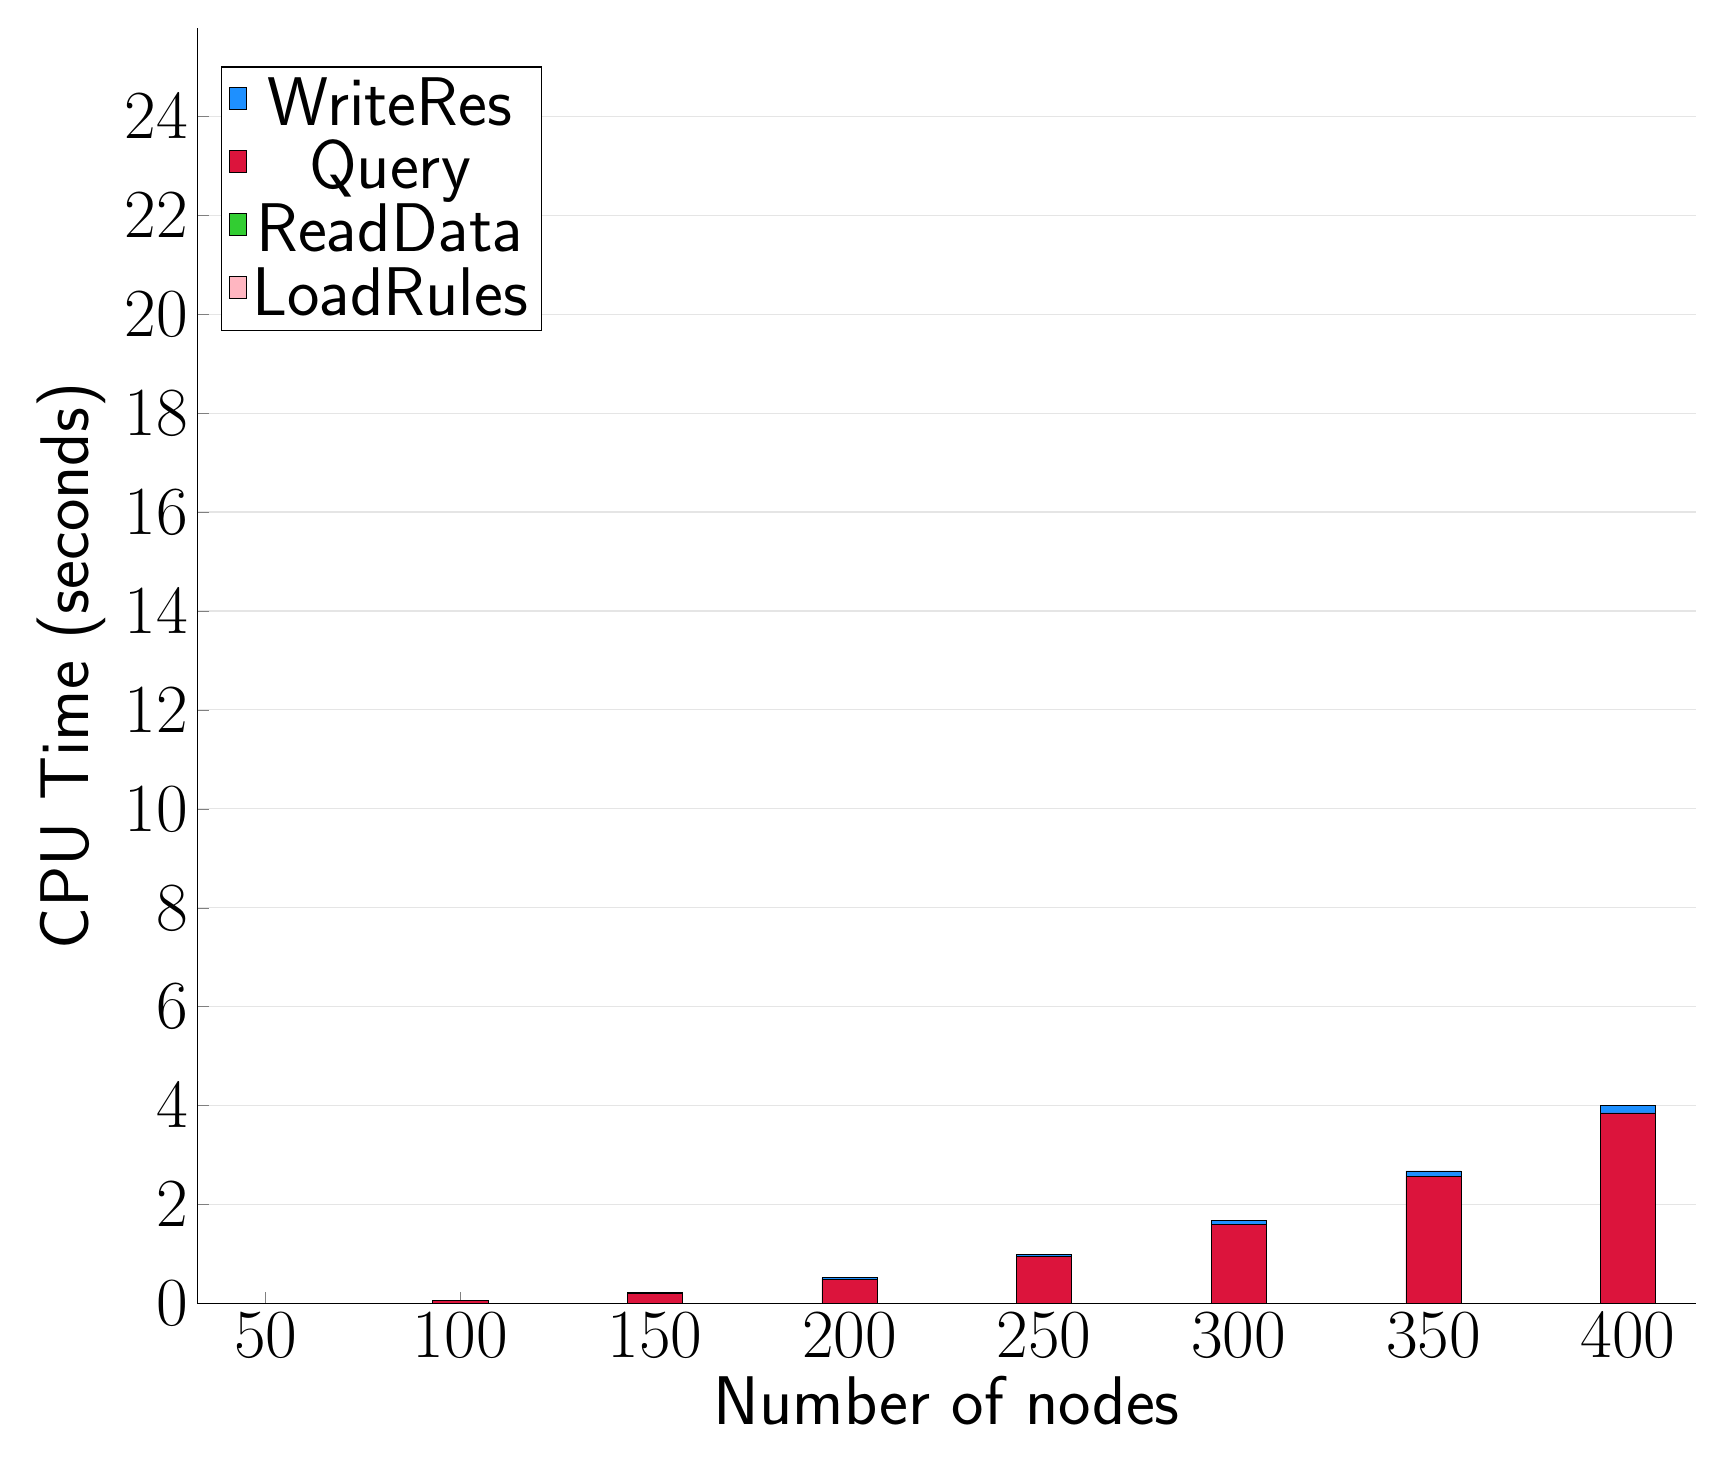
\begin{tikzpicture}
\begin{axis}[
   ybar stacked,
   width=1.7\textwidth,
   bar width=0.7cm,
   ymajorgrids, tick align=inside,
   major grid style={draw=gray!20},
   xtick=data,
   ymin=0, ymax=25.779619999999998,
   axis x line*=bottom,
   axis y line*=left,
   enlarge x limits=0.05,
   legend style={
       at={(0.23, 0.97)},
       anchor=north east,
       legend columns=1,
       font=\Huge,
   },
   ylabel={CPU Time (seconds)},
   xlabel={Number of nodes},
   label style={font=\Huge},
   tick label style={font=\Huge},
]
\addlegendimage{fill=DodgerBlue, draw=black, line width=0.2pt}
\addlegendentry{WriteRes}
\addlegendimage{fill=Crimson, draw=black, line width=0.2pt}
\addlegendentry{Query}
\addlegendimage{fill=LimeGreen, draw=black, line width=0.2pt}
\addlegendentry{ReadData}
\addlegendimage{fill=LightPink, draw=black, line width=0.2pt}
\addlegendentry{LoadRules}
\addplot +[fill=LightPink, draw=black, line width=0.2pt] coordinates {
(50, 0.0006127000000000001)
(100, 0.0005970000000000003)
(150, 0.0006277999999999998)
(200, 0.0006027000000000001)
(250, 0.0006254000000000001)
(300, 0.0006182000000000002)
(350, 0.0006183999999999996)
(400, 0.0006082000000000003)
};
\addplot +[fill=LimeGreen, draw=black, line width=0.2pt] coordinates {
(50, 0.00017659999999999958)
(100, 0.0002153999999999995)
(150, 0.0002685999999999998)
(200, 0.0003018999999999996)
(250, 0.0003526999999999997)
(300, 0.00040639999999999947)
(350, 0.0004432000000000007)
(400, 0.0004793999999999995)
};
\addplot +[fill=Crimson, draw=black, line width=0.2pt] coordinates {
(50, 0.007602300000000001)
(100, 0.06051260000000001)
(150, 0.2072289)
(200, 0.48774570000000006)
(250, 0.9499592)
(300, 1.6064833)
(350, 2.5673429000000003)
(400, 3.8520795)
};
\addplot +[fill=DodgerBlue, draw=black, line width=0.2pt] coordinates {
(50, 0.0023033999999999997)
(100, 0.0092248)
(150, 0.021591100000000005)
(200, 0.03815340000000001)
(250, 0.051117000000000024)
(300, 0.07741620000000005)
(350, 0.11364100000000006)
(400, 0.1485033000000001)
};
\end{axis}
\end{tikzpicture}

\end{document}
